\subsection{High-contrast imaging with the apodizing phase plate}
\label{ssec:algo_app_imaging}

LM-band imaging data taken with the apodizing phase plate undergo the
same basic reduction as standard imaging data. \TODO{Does this include
  background subtraction or is the background subtracted during the
  ADI processing?}



\begin{enumerate}
\item Locate the positions of the PSFs with respect to each other
  (dither correction).
\item Center the leakage PSF in the frames.
\item Extract the coronagraphic PSFs and combine them into a single
  cube (see Fig.~\ref{fig:app_psf_combine}). This has almost
  360\degr\ dark zones.
\item Median combine the cube to obtain the reference PSF image.
\item Subtract PSF image from all layers of the cube.
\item Derotate all layers to correct for field rotation, taking into
  account a static mask to reject noisy border regions of the dark
  zones.
\item Sum the layers to obtain final image.
\end{enumerate}

\begin{figure}
  \centering
  \resizebox{0.8\textwidth}{!}{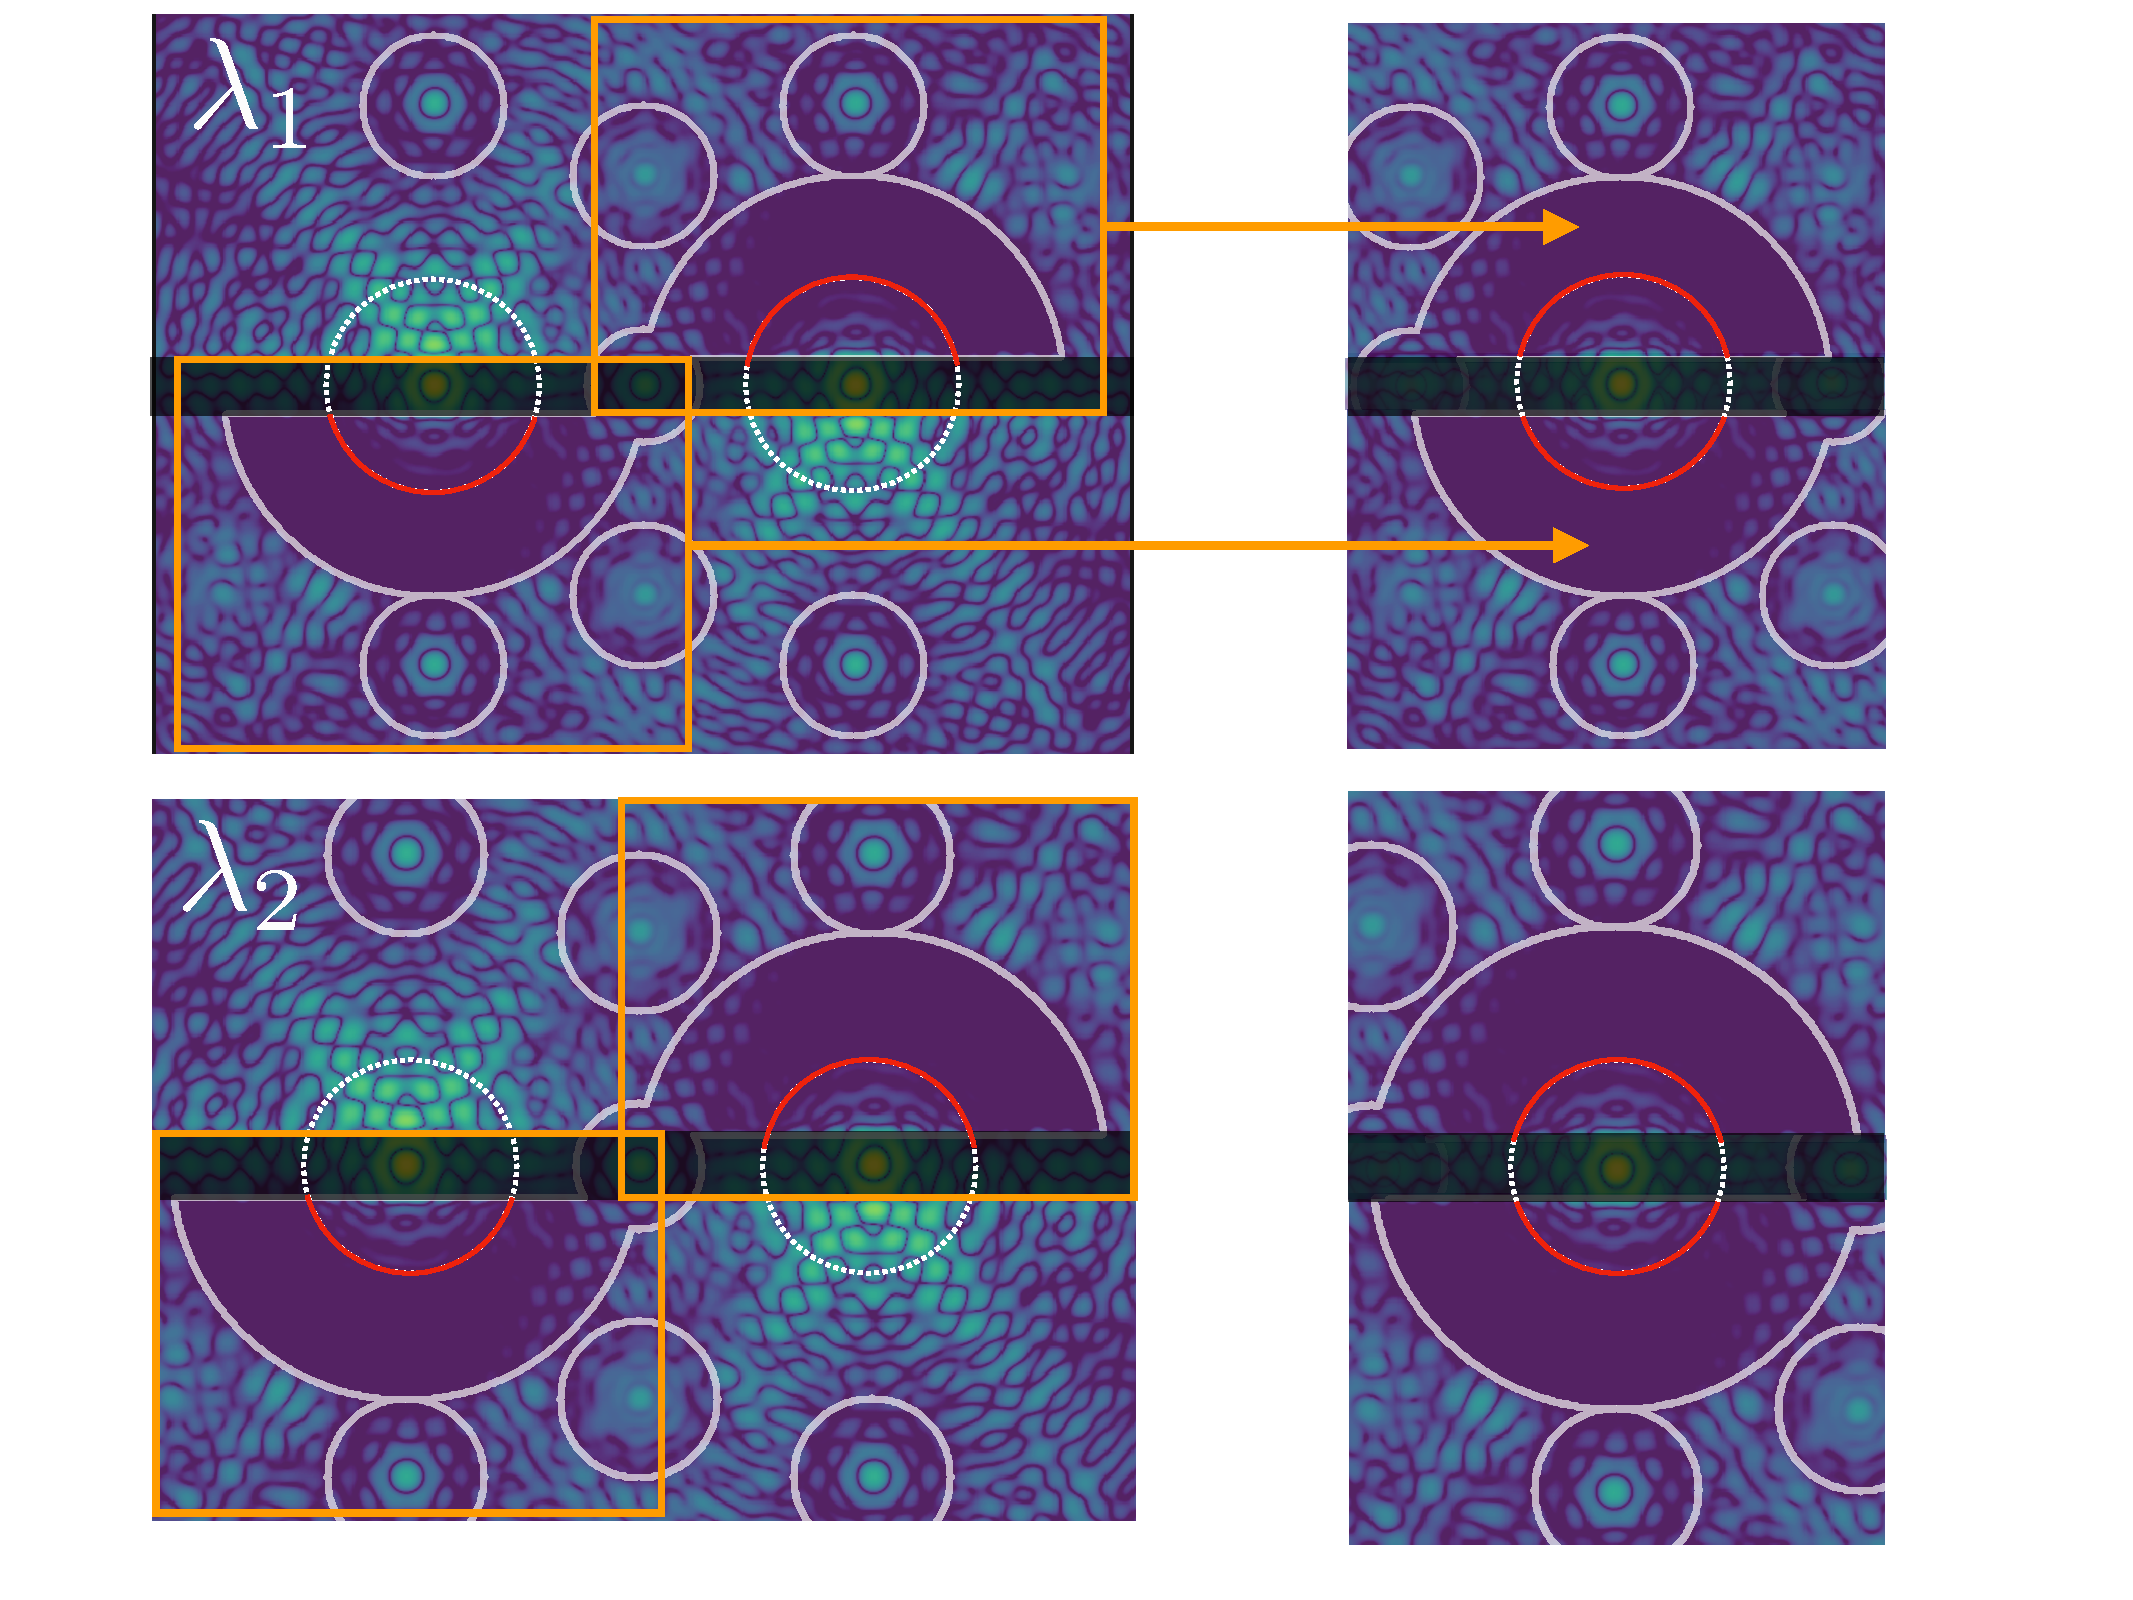
\includegraphics{vAPP_data_reduction}}
  \caption{Combination of the coronagraphic PSFs of APP observations
    into a single PSF with 360\degr\ dark zones. \TODO{This is a figure
      by David Doelman. The layout of the PSFs is not what we expect
      for METIS, therefore needs to be updated.}}
  \label{fig:app_psf_combine}
\end{figure}

%%% Local Variables:
%%% TeX-master: "METIS_DRLD"
%%% End:
